\chapter[État de l'Art]{État de l'Art de la Détection d'Anomalies Vibratoires par TinyML}
\label{chap:etat_art}
\thispagestyle{plain}

\section{Introduction}
\label{sec:intro_etat_art}

Dans le contexte de l'Industrie 4.0, la maintenance prédictive (PdM) est devenue un impératif stratégique visant à garantir la fiabilité et la continuité de la production \cite{hector2024,achouch2022}. La PdM, en s'appuyant sur des algorithmes avancés, permet d'anticiper les défaillances des équipements rotatifs, dont l'état est principalement évalué par la surveillance vibratoire \cite{ran2019}. Traditionnellement, l'analyse des données d'intelligence artificielle (IA) s'effectuait sur des serveurs distants ou dans le \textit{cloud}, imposant des contraintes de latence, de bande passante et de coût \cite{njor2024}.

Le paradigme du TinyML (\textit{Tiny Machine Learning}) apporte une solution disruptive en déplaçant l'inférence des modèles d'apprentissage automatique (ML) directement sur le dispositif embarqué (\textit{Edge}) \cite{tsoukas2024}. Cette approche permet la détection d'anomalies en temps réel au plus près de la source de données, même dans des environnements contraints. Le présent chapitre propose un état de l'art structuré autour de quatre axes majeurs : l'évolution des stratégies de maintenance, les fondements de l'analyse vibratoire, les méthodologies de détection d'anomalies par apprentissage automatique, et l'application du paradigme TinyML dans le secteur industriel.

\section{Stratégies de maintenance}
\label{sec:strategies_maintenance}

L'évolution des pratiques de maintenance industrielle est marquée par une quête constante d'optimisation des coûts et d'amélioration de la fiabilité des systèmes, progressant d'une approche réactive à une stratégie proactive et anticipative \cite{ran2019}. La normalisation, notamment par la norme européenne EN 13306:2017, fournit un cadre terminologique essentiel pour distinguer ces stratégies \cite{en13306}.

\subsection{Typologie de la maintenance industrielle}

La norme EN 13306 \cite{en13306} et les travaux de revue \cite{ran2019} définissent principalement trois grandes catégories d'actions de maintenance :

\textbf{Maintenance Corrective (RM -- Reactive Maintenance) :} Il s'agit de la stratégie la plus élémentaire, exécutée uniquement après qu'une défaillance se soit produite et que l'équipement soit dans un état défectueux \cite{en13306,ran2019}. Bien que simple à mettre en œuvre pour les actifs non critiques, elle entraîne inévitablement des temps d'arrêt imprévus, des coûts de réparation élevés, estimés jusqu'à trois fois supérieurs à ceux d'une maintenance planifiée, et des risques de dommages collatéraux \cite{ran2019}.

\textbf{Maintenance Préventive (PM -- Preventive Maintenance) :} Cette stratégie vise à éviter la panne en planifiant des interventions à des intervalles prédéterminés (basés sur le temps ou l'usage) ou selon une condition prédéfinie \cite{en13306,ran2019}. La maintenance préventive systématique réduit l'aléa mais présente l'inconvénient d'un risque de sur-entretien coûteux, où des composants sont remplacés avant que leur durée de vie utile ne soit atteinte \cite{ran2019}.

\textbf{Maintenance Prédictive (PdM -- Predictive Maintenance) :} La PdM représente la forme la plus évoluée de maintenance conditionnelle (CBM) \cite{achouch2022,lee2014,jardine2006}. Elle s'appuie sur la surveillance de l'état réel de l'équipement (\textit{condition monitoring}) pour prédire le moment futur de la défaillance. La PdM permet d'optimiser l'intervalle de maintenance (\textit{adaptive intervals}) en fonction de l'état de santé du système, assurant une intervention juste à temps.

\textit{Note} : Selon EN 13306, la PdM est techniquement un sous-ensemble de la CBM. Cette étude adopte la classification tripartite courante pour clarté pédagogique.

La \textbf{Maintenance Conditionnelle (CBM)}, définie par l'ISO 17359 \cite{iso17359}, fonde ses décisions sur l'observation des indicateurs de l'état de l'équipement. La CBM est considérée comme un précurseur de la PdM. La PdM étend la CBM par l'intégration d'outils d'analyse avancée (ML/DL) pour effectuer le \textbf{Pronostic} (prédiction de l'évolution de la dégradation et de la Durée de Vie Résiduelle, RUL) en plus du \textbf{Diagnostic} (identification de la cause de la panne). Le cadre d'ingénierie qui intègre ces deux tâches est appelé \textit{Prognostics and Health Management} (PHM) \cite{lee2014,achouch2022}.

\begin{figure}[ht]
\centering
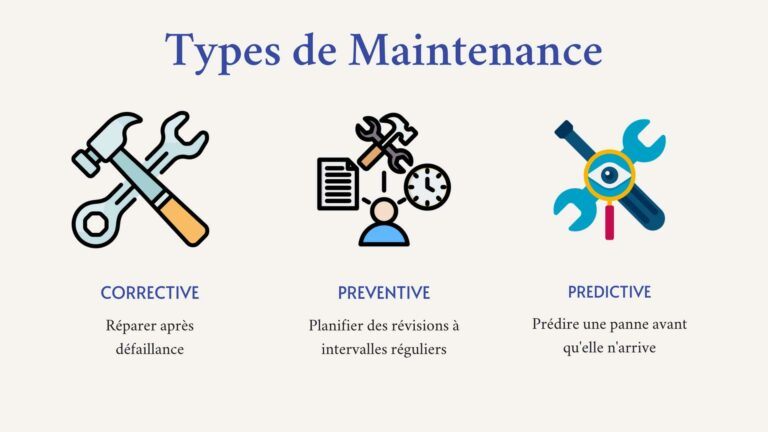
\includegraphics[width=0.85\textwidth]{images/types-de-maintenance.jpg}
\caption{Types de maintenance industrielle}
\label{fig:maintenance_evolution}
\end{figure}

\subsection{Enjeux économiques des temps d'arrêt}

Les temps d'arrêt imprévus (\textit{unplanned downtime}) constituent un enjeu économique majeur pour l'industrie manufacturière. Selon une analyse sectorielle réalisée par Siemens en 2024, basée sur une enquête auprès de 181 professionnels de la maintenance entre 2019 et 2023, les coûts horaires d'immobilisation varient considérablement selon le secteur \cite{siemens2024}\footnote{Ces données proviennent d'un rapport industriel (Siemens Senseye, 2024) et n'ont pas fait l'objet d'une validation académique indépendante par des revues évaluées par les pairs. Elles sont utilisées ici pour contextualiser l'enjeu stratégique de la maintenance prédictive.} :

\begin{itemize}
\item Biens de consommation courante (FMCG) : 36\,000\,\$/heure
\item Industrie automobile : jusqu'à 2,3\,millions\,\$/heure dans les grandes usines
\item Petites et moyennes entreprises : environ 150\,000\,\$/heure
\end{itemize}

À l'échelle macroéconomique, les pertes annuelles attribuées aux temps d'arrêt non planifiés pour les 500 plus grandes entreprises mondiales sont estimées à 1,4~trillion de dollars \cite{siemens2024}. Le potentiel d'économie associé à l'adoption de la Maintenance Prédictive (PdM) est régulièrement chiffré dans les rapports industriels à une réduction des coûts de maintenance de l'ordre de 40\,\% \cite{siemens2024}. Ces projections, si elles se confirment à grande échelle, représenteraient des économies significatives pour les entreprises industrielles.

\subsection{Défis pour les PME et positionnement du projet}

Malgré le potentiel économique de la PdM, les solutions traditionnelles d'IA et d'IoT restent complexes et coûteuses à déployer, notamment pour les PME \cite{siemens2024}. Ces dernières font face à des barrières significatives pour l'adoption de la maintenance prédictive \cite{oecd2021} :
\begin{itemize}
\item Coût prohibitif des solutions commerciales (>5\,000\,€)
\item Absence d'expertise IA/IoT interne
\item ROI incertain pour équipements auxiliaires
\end{itemize}

Le paradigme TinyML, en permettant l'implémentation de modèles ML directement sur des microcontrôleurs à faible coût, pourrait offrir une alternative plus accessible pour la détection d'anomalies vibratoires. Cette approche vise à démocratiser l'accès à la maintenance prédictive pour les entreprises disposant de ressources limitées.

\section{Analyse vibratoire}
\label{sec:analyse_vibratoire}

L'analyse vibratoire est la modalité de surveillance la plus courante et la plus performante pour le \textit{Condition Monitoring} des machines tournantes, car la vibration est la modalité de référence standardisée pour l'évaluation de l'état de ces équipements (ISO 20816/17359) \cite{iso20816-1,hassan2024}. Les défauts mécaniques tels que le désalignement, le balourd, les roulements endommagés ou les défauts d'engrenage génèrent des signatures distinctes dans les signaux vibratoires \cite{tiboni2022}.

\subsection{Cadre normatif et évaluation}

L'évaluation des vibrations est encadrée par les normes internationales de l'Organisation Internationale de Normalisation (ISO), notamment la série ISO 20816.

La \textbf{Norme ISO 20816-1:2016} \cite{iso20816-1} établit les lignes directrices générales pour la mesure et l'évaluation des vibrations mécaniques des machines, applicable aux mesures effectuées sur les parties tournantes (arbres) et non tournantes (paliers) en conditions de fonctionnement stable. Elle stipule que l'évaluation se fait typiquement en considérant l'amplitude de la vibration large bande observée. Elle précise également les quantités de mesure (déplacement, vitesse, accélération) et la plage de réponse en fréquence requise, qui est d'au moins 10\,Hz à 1\,000\,Hz pour l'évaluation de la vitesse efficace (r.m.s.).

La \textbf{Norme ISO 20816-3:2022} \cite{iso20816-3} est un document sectoriel qui spécifie les exigences pour l'évaluation des vibrations des machines industrielles accouplées d'une puissance nominale supérieure à 15\,kW et fonctionnant entre 120\,tr/min et 30\,000\,tr/min. Elle fournit des critères d'évaluation pour les mesures effectuées \textit{in-situ} sur des paliers ou des supports de palier.

Par ailleurs, la \textbf{Norme ISO 17359:2018} \cite{iso17359} fournit les lignes directrices pour l'établissement d'un programme de surveillance d'état (CBM), incluant la sélection des variables à mesurer et la détermination des critères d'alarme.

\subsection{Acquisition de données et capteurs}

L'acquisition des données vibratoires est généralement assurée par des accéléromètres \cite{hassan2024}. Historiquement, des capteurs piézoélectriques industriels ont été utilisés, mais la tendance pour les dispositifs IoT et TinyML est à l'intégration d'accéléromètres basés sur la technologie \textbf{MEMS} (\textit{Micro-Electro-Mechanical Systems}). Les capteurs MEMS sont privilégiés pour leur faible coût, leur petite taille et leur faible consommation d'énergie, ce qui les rend idéaux pour les systèmes embarqués contraints \cite{hassan2024,arciniegas2025}.

\subsection{Traitement du signal et extraction de caractéristiques}

Le signal vibratoire brut capturé doit subir un traitement pour en extraire des caractéristiques pertinentes pour le diagnostic. Ce processus suit typiquement une chaîne en plusieurs étapes:

\begin{enumerate}
\item \textbf{Pré-traitement :} Il inclut le nettoyage des données brutes pour réduire le bruit et les artefacts \cite{bagri2024}.
\item \textbf{Traitement du Signal :} C'est la conversion du signal du domaine temporel au domaine fréquentiel ou temps-fréquence.
\item \textbf{Extraction de Caractéristiques :} Calcul d'indicateurs (statistiques, fréquentiels) qui servent d'entrées aux modèles ML/DL.
\end{enumerate}

\textbf{Analyse Temporelle :} L'analyse du domaine temporel examine directement la forme d'onde enregistrée pour en extraire des descripteurs statistiques. Le niveau d'amplitude est un bon indicateur de la condition de la machine et de la gravité du défaut. Les caractéristiques couramment utilisées incluent :
\begin{itemize}
\item \textbf{La Moyenne Quadratique (RMS -- Root Mean Square) :} Mesure robuste de l'amplitude de la vibration qui est moins sensible aux variations extrêmes et plus indicative de l'énergie totale du signal.
\item \textbf{Le Kurtosis (Aplatissement) :} Indicateur statistique de la distribution des pics. Un Kurtosis élevé peut signaler des défauts précoces dans les roulements.
\end{itemize}

\textbf{Analyse Fréquentielle (FFT) :} La Transformation de Fourier Rapide (FFT), introduite par Cooley et Tukey \cite{cooley1965}, convertit le signal temporel en spectre de fréquences pour identifier les \textbf{fréquences caractéristiques} des défauts (par exemple, balourd près de $1 \times F_r$, désalignement près de $2 \times F_r$, où $F_r$ est la fréquence de rotation).

\textbf{Théorème de Nyquist :} Le théorème impose une fréquence d'échantillonnage $f_s \geq 2f_{max}$ pour éviter l'aliasing. La norme ISO 20816-1 spécifie typiquement une analyse jusqu'à 1\,kHz pour les machines tournantes \cite{iso20816-1}.

\textbf{Fenêtrage et paramètres FFT :} Des fonctions de fenêtrage (Hann, Hamming) sont appliquées pour réduire les fuites spectrales. Le choix du nombre de points FFT ($N$) résulte d'un compromis entre résolution fréquentielle ($\Delta f = f_s/N$) et latence de calcul. Les détails de configuration et d'optimisation relèvent de la méthodologie expérimentale (Chapitre~\ref{chap:conception}).

\subsection{Caractéristiques vibratoires courantes}

L'efficacité de la détection d'anomalies dépend de l'extraction de caractéristiques pertinentes. La littérature identifie deux catégories principales \cite{ran2019,tiboni2022} :

\textbf{Domaine temporel :} Les indicateurs statistiques caractérisent l'amplitude et la distribution du signal vibratoire :
\begin{itemize}
\item \textbf{RMS (Root Mean Square) :} $\sqrt{\frac{1}{N}\sum_{i=1}^{N}x_i^2}$ -- Indicateur d'usure générale et d'énergie totale
\item \textbf{Valeur crête et facteur de crête :} $\max(|x_i|)$ et $\frac{\text{Crête}}{\text{RMS}}$ -- Sensibles aux chocs et défauts localisés
\item \textbf{Kurtosis :} $\frac{\sum(x_i-\bar{x})^4}{N\sigma^4}$ -- Détection précoce de défauts de roulements
\item \textbf{Asymétrie (Skewness) :} $\frac{\sum(x_i-\bar{x})^3}{N\sigma^3}$ -- Indicateur de désalignement
\end{itemize}

\textbf{Domaine fréquentiel :} L'analyse spectrale permet d'identifier la nature du défaut par ses fréquences caractéristiques :
\begin{itemize}
\item \textbf{Pics harmoniques :} Amplitude à $1 \times F_r$ (balourd), $2 \times F_r$ (désalignement), où $F_r$ est la fréquence de rotation
\item \textbf{Énergie spectrale par bandes :} Basses fréquences (défauts mécaniques), hautes fréquences (défauts de roulements)
\item \textbf{Enveloppe spectrale :} Démodulation d'amplitude pour détecter les défauts de roulements
\end{itemize}


\section{Détection d'anomalies par Apprentissage Automatique}
\label{sec:detection_anomalies}

L'apprentissage automatique (ML) est au cœur de la PdM pour l'identification et la classification autonomes des schémas de comportement anormaux \cite{achouch2022,chandola2009}. Le choix de la méthode dépend crucialement de la disponibilité de données étiquetées de défaillance, souvent rares en environnement industriel.

\subsection{Approches non supervisées et semi-supervisées}

Les méthodes non supervisées sont essentielles pour la détection d'anomalies (AD) dans les scénarios industriels où la majorité des données représentent un fonctionnement normal (état sain) \cite{arciniegas2025}. Ces algorithmes modélisent le comportement normal et signalent tout écart significatif.

\textbf{K-means} \cite{macqueen1967,chandola2009} : Méthode de partitionnement non supervisée qui regroupe des observations présentant des caractéristiques proches. En maintenance, elle sert à modéliser la \textbf{normalité} et à signaler comme \textbf{anomalies} les observations très éloignées des centroïdes. Atouts : simplicité, faible empreinte mémoire, interprétabilité. Points d'attention : hypothèse de clusters compacts, choix de $k$ (typiquement par méthode du coude).

\textbf{Isolation Forest (IF) :} Cet algorithme, particulièrement efficace pour l'AD, isole les anomalies en utilisant des partitions aléatoires. Il est performant et nécessite une complexité moyenne ($O(n \log n)$), le rendant adapté à l'embarqué. Antonini et al. (2023) l'ont utilisé sur microcontrôleur, réalisant une détection d'anomalie en moins de 16\,ms avec 84\,KB de RAM \cite{antonini2023}.

\textbf{Autoencodeurs (AE) :} Les autoencodeurs sont des réseaux neuronaux non supervisés entraînés à reconstruire les données d'entrée. Ils excellent à modéliser la \textit{normalité}. Une erreur de reconstruction élevée indique une anomalie \cite{ran2019}. Les AE sont utilisés pour la détection d'anomalies dans la maintenance prédictive, notamment en environnement \textit{Edge}.

\subsection{Approches supervisées et \textit{Deep Learning} (DL)}

Les méthodes supervisées sont utilisées lorsque des jeux de données de défaillance étiquetées sont disponibles, ce qui permet des tâches de classification et de diagnostic plus précises.

\textbf{Machines à Vecteurs de Support (SVM) :} Les SVM sont couramment employés pour la classification des défauts vibratoires \cite{jemmali2021,ran2019}. Elles offrent une précision élevée mais leur complexité est généralement quadratique ($O(n^2)$), ce qui peut être gourmand en mémoire pour l'implémentation embarquée.

\textbf{Forêts Aléatoires (RF) :} Les RF sont également utilisés pour le diagnostic. Leur performance est jugée bonne dans les benchmarks \cite{bagri2024}.

L'avènement du \textit{Deep Learning} (DL) a permis d'améliorer la précision en exploitant directement les signaux bruts ou les représentations temps-fréquence sans nécessiter une extraction manuelle de caractéristiques sophistiquée.

\textbf{Réseaux Neuronaux Convolutifs (CNN) :} Les CNN, notamment les variantes 1D (CNN-1D) adaptées aux séries temporelles vibratoires, sont très efficaces pour extraire des caractéristiques locales \cite{bagri2024,langer2025}. Langer et al. (2025) ont démontré, dans leur étude, une latence de 84,5\,ms pour un CNN optimisé sur microcontrôleur \cite{langer2025}.

\textbf{Mémoires à Long Terme et Court Terme (LSTM) :} Les réseaux récurrents (RNN) et leurs variantes comme les LSTM ou les GRU (Gated Recurrent Units) sont idéaux pour capturer les dépendances temporelles des données de dégradation \cite{ran2019,bagri2024}. Cependant, ils exigent une utilisation de mémoire élevée, limitant leur déploiement sur les microcontrôleurs ultra-contraints \cite{gupta2025}.

La comparaison objective des algorithmes met en évidence un compromis crucial : les méthodes DL offrent la meilleure précision mais la plus haute complexité et les besoins en mémoire les plus importants, tandis que les méthodes non supervisées comme K-means ou Isolation Forest offrent un équilibre optimal pour le déploiement sur microcontrôleurs.

\begin{table}[ht]
\centering
\caption{Comparaison qualitative des méthodes de détection d'anomalies}
\label{tab:ml_comparison}
\begin{tabular}{p{2.8cm}p{2.5cm}p{4.2cm}p{3.2cm}p{2cm}}
\toprule
\textbf{Famille} &
\textbf{Adéquation PdM} &
\textbf{Usage typique} &
\textbf{Points d'attention} &
\textbf{Réf.} \\
\midrule

K-means &
Bonne (léger, simple) &
Modéliser la normalité; score distance-centroïdes &
Choix de $k$, sensibilité à l'échelle &
\cite{macqueen1967,chandola2009} \\
\midrule

Isolation Forest &
Bonne si anomalies rares &
Isolement par partitions aléatoires &
Réglages (\#arbres/profondeur) &
\cite{chandola2009,antonini2023} \\
\midrule

One-Class SVM &
Moyenne &
Frontière de normalité &
Sensible aux hyperparamètres/échelle &
\cite{chandola2009} \\
\midrule

Autoencodeurs &
Possible (optimisés) &
Reconstruction du normal &
Empreinte/mise au point des seuils &
\cite{chandola2009,ran2019} \\
\midrule

CNN/LSTM &
Possible (quantifiés) &
Extraction automatique de caractéristiques &
Ressources élevées, quantification requise &
\cite{langer2025,arciniegas2025} \\

\bottomrule
\multicolumn{5}{p{15cm}}{\small Note : Les performances dépendent fortement de la configuration matérielle, des paramètres DSP et des compromis algorithmiques. Validation spécifique requise pour chaque contexte.} \\
\end{tabular}
\end{table}


\section{TinyML Industriel}
\label{sec:tinyml_industriel}

Le TinyML est l'extension de l'intelligence artificielle jusqu'aux dispositifs d'extrémité (\textit{extreme edge}), permettant l'exécution de modèles ML directement sur des microcontrôleurs (MCU) à ultra-faible consommation \cite{tsoukas2024,njor2024}. Ce changement de paradigme est fondamental pour la PdM, car il supprime les dépendances à la connectivité réseau et réduit drastiquement la latence.

\subsection{Définition et Contraintes Techniques}

Le TinyML se déploie généralement sur des MCU 32-bit caractérisés par des ressources matérielles extrêmement limitées. Les contraintes typiques sont sévères :
\begin{itemize}
\item \textbf{Mémoire vive (SRAM) :} Typiquement inférieure à 256\,KB.
\item \textbf{Mémoire flash (Stockage) :} Habituellement limitée (quelques MB).
\item \textbf{Consommation énergétique :} Faible, souvent de l'ordre du milli-watt.
\end{itemize}

Ces contraintes imposent l'utilisation de modèles ML extrêmement légers. L'objectif principal est de permettre une inférence en temps réel avec une latence minimale. Il est important de distinguer deux métriques :
\begin{itemize}
\item \textbf{Latence d'inférence :} Le temps de calcul du modèle ML uniquement, typiquement visé à moins de 10\,ms pour les applications critiques.
\item \textbf{Latence système totale :} Incluant acquisition des données, pré-traitement, inférence et génération d'alerte, généralement inférieure à 100\,ms, ce qui reste compatible avec les exigences industrielles de surveillance en temps réel.
\end{itemize}

\subsection{Chaîne d'outils et Optimisation}

Les déploiements TinyML s'appuient sur des moteurs d'inférence pour microcontrôleurs, des pipelines de traitement du signal (DSP) et des techniques d'optimisation pour réduire l'empreinte mémoire et la latence tout en maintenant la performance de détection.

\textbf{Moteurs d'inférence :} Parmi les frameworks disponibles, \textbf{TensorFlow Lite Micro} permet la conversion et l'exécution de modèles entraînés sur PC vers des microcontrôleurs \cite{tsoukas2024}. D'autres solutions incluent des implémentations spécifiques aux fabricants de MCU.

\textbf{Plateformes de développement :} Des environnements intégrés comme \textbf{Edge Impulse} proposent une chaîne complète (acquisition, traitement DSP, apprentissage, déploiement) avec génération de bibliothèques embarquées. Ces plateformes intègrent généralement :

\begin{itemize}
\item Support de multiples architectures MCU (ESP32, STM32, Arduino, etc.)
\item Algorithmes d'apprentissage (clustering, classification, réseaux neuronaux)
\item Pipelines DSP (FFT, transformées temps-fréquence)
\item Outils de quantification (int8/int16) pour la compression des modèles
\end{itemize}

Des études de cas rapportent l'utilisation de ces plateformes pour la détection vibratoire, avec des résultats variables selon la configuration matérielle et les compromis algorithmiques adoptés \cite{arciniegas2025}.

L'optimisation des modèles repose principalement sur des techniques de compression :
\begin{itemize}
\item \textbf{Quantification :} Réduction de la précision numérique des poids (par exemple, de 32 bits flottants à 8 bits entiers), réduisant la taille du modèle et accélérant l'inférence \cite{arciniegas2025,langer2025}.
\item \textbf{Élagage (\textit{Pruning}) :} Suppression des connexions et neurones non essentiels pour réduire la complexité \cite{tsoukas2024}.
\end{itemize}

\subsection{Cas d'application en détection d'anomalies vibratoires}

Des travaux récents démontrent la \textbf{faisabilité} de la détection d'anomalies vibratoires en temps quasi réel sur microcontrôleurs, avec des approches et performances variables selon les configurations matérielles et algorithmiques :

\textbf{Antonini et al. (2023)} \cite{antonini2023} ont validé un système basé sur \textbf{Isolation Forest} sur microcontrôleur \textbf{ESP32\_WROVER\_IE} (avec mémoire externe PSRAM), démontrant une robustesse en environnements industriels extrêmes (-40°C à +85°C) avec des latences d'inférence de l'ordre de quelques dizaines de millisecondes.

\textbf{Note matérielle :} Ces résultats ont été obtenus sur une configuration disposant de mémoire externe (PSRAM); la transposabilité dépend des ressources disponibles sur le microcontrôleur cible.

D'autres études \cite{arciniegas2025,langer2025,gupta2025} rapportent des implémentations TinyML utilisant des réseaux neuronaux quantifiés (CNN-1D) pour la détection vibratoire, avec des précisions variables en laboratoire. Les performances dépendent fortement du \textbf{contexte matériel}, des \textbf{paramètres DSP} (taille FFT, fenêtrage) et des \textbf{compromis mémoire/latence} adoptés.

Le TinyML permet théoriquement le déport d'une capacité analytique sophistiquée (y compris \textit{Deep Learning} ou algorithmes d'ensemble) directement sur des dispositifs peu coûteux et autonomes, visant une détection d'anomalies à faible latence potentiellement compatible avec les exigences industrielles en temps réel.

Il est important de reconnaître que la majorité des travaux académiques sur le TinyML pour la maintenance s'appuient sur des validations en laboratoire avec des défauts contrôlés. Cette approche méthodologique, bien que nécessaire pour établir la faisabilité technique, constitue une première étape vers le déploiement industriel. Les défis de la maintenance à long terme et l'adaptation aux conditions industrielles variables restent des axes de recherche ouverts pour l'ensemble de la communauté scientifique. De plus, le compromis fondamental entre latence et précision reste sous-exploré : une latence réduite (<10\,ms) implique souvent des simplifications algorithmiques (réduction du nombre de caractéristiques, quantification agressive) qui peuvent affecter la sensibilité de détection, particulièrement pour les anomalies subtiles ou progressives caractéristiques de l'usure normale des équipements industriels.

\section{Synthèse critique et positionnement}
\label{sec:synthese_critique}

L'analyse de l'état de l'art confirme que la Maintenance Prédictive (PdM) est un impératif économique pour l'industrie, essentiel pour contrecarrer les coûts prohibitifs des arrêts non planifiés (variant de 36\,000\,\$ à 2,3 millions de dollars par heure selon le secteur \cite{siemens2024}). La surveillance vibratoire, encadrée par les normes ISO 20816, est la méthode de prédilection, avec une complexité d'analyse gérable grâce à l'extraction de caractéristiques fréquentielles (FFT).

Le paradigme TinyML offre une opportunité prometteuse pour explorer des approches d'IA plus accessibles pour les systèmes de surveillance contraints. Les études de cas récentes (Antonini 2023, Arciniegas 2025, Langer 2025) ont démontré la faisabilité technique de la détection d'anomalies en temps réel (<100\,ms) en utilisant des microcontrôleurs et des modèles optimisés \cite{antonini2023,arciniegas2025,langer2025}.

Cependant, plusieurs lacunes et considérations critiques persistent dans la littérature :

\begin{enumerate}
\item \textbf{Accessibilité PME :} La documentation des implémentations "clés en main" pour les techniciens de maintenance des PME, dépourvus d'expertise en IA, reste limitée \cite{oecd2021}.

\item \textbf{Transition Lab-Terrain :} Le passage de la validation académique au déploiement industriel reste un défi majeur. Les méthodologies pour adapter les modèles développés en laboratoire aux conditions opérationnelles réelles nécessitent davantage de recherche collaborative industrie-université.

\item \textbf{Standardisation des Métriques :} Il existe un manque de \textit{benchmarks} TinyML standardisés spécifiquement pour la maintenance prédictive vibratoire. Les métriques de validation doivent inclure non seulement la précision globale, mais aussi la précision, le rappel, et le score F1, particulièrement important pour évaluer la détection des anomalies rares. MLPerf Tiny, bien qu'existant, se concentre sur d'autres applications \cite{banbury2021}.

\item \textbf{Considérations de Sécurité :} Un aspect critique sous-exploré est la gestion des faux négatifs. Un système de maintenance prédictive doit intégrer des mécanismes de fail-safe pour éviter les défaillances catastrophiques en cas d'anomalie non détectée. Une approche à seuils multiples avec alertes progressives est recommandée.

\item \textbf{Comparaison Baseline :} Les études actuelles manquent souvent de comparaison avec les méthodes traditionnelles (inspection manuelle, maintenance préventive calendaire) en termes de coût/efficacité, rendant difficile l'évaluation du gain réel pour les PME.

\item \textbf{Détails d'Optimisation :} Les détails précis de l'optimisation des flux de données et des modèles (quantification, gestion mémoire dynamique) pour les architectures MCU ultra-contraintes ne sont pas toujours divulgués dans les publications académiques, complexifiant la reproduction des performances.
\end{enumerate}

\textbf{Positionnement critique :} L'analyse de l'état de l'art révèle un décalage entre le potentiel économique théorique de la PdM (économies projetées de 40\,\% des coûts de maintenance selon les rapports industriels \cite{siemens2024}) et les défis pratiques du déploiement TinyML sur microcontrôleurs contraints. Les contraintes matérielles (mémoire limitée, puissance de calcul réduite) imposent des compromis algorithmiques qui peuvent affecter la précision de détection. De plus, la majorité des validations expérimentales publiées s'appuient sur des conditions de laboratoire avec des défauts contrôlés \cite{antonini2023,arciniegas2025,langer2025}, laissant ouverte la question de la robustesse en environnement industriel réel avec variabilité des charges, conditions environnementales, et modes de dégradation progressifs.

Ces lacunes identifiées orientent vers le développement de solutions adaptées aux contraintes industrielles réelles, dont la conception sera détaillée dans le chapitre suivant.